%%%%%%%%%%%%%%%%%%%%%%%%%%%%%%%%%%%%%%%%%%%%%%%%%%%%%%%%%%%%%%%%%%%%%%%%%%%%%%%%%%%%%%%%%%%%%%%%%%%%%%%%%
%%%%%  Topic 2 -- Edge Computing                                                                    %%%%%
%%%%%  Part of the Module 1 study material; compile main.tex for the full set,                      %%%%%
%%%%%  or this file on its own (it is a subfile and picks up ../preamble.tex).                      %%%%%
%%%%%                                                                                               %%%%%
%%%%%  Syllabus coverage: Introduction, Need for Edge Computing, Edge Computing Architecture,       %%%%%
%%%%%  Cloud vs. Edge Computing, Applications.                                                      %%%%%
%%%%%%%%%%%%%%%%%%%%%%%%%%%%%%%%%%%%%%%%%%%%%%%%%%%%%%%%%%%%%%%%%%%%%%%%%%%%%%%%%%%%%%%%%%%%%%%%%%%%%%%%%
\documentclass[../main.tex]{subfiles}

\begin{document}

\topic{Edge Computing}

\begin{tabularx}{\textwidth}{@{}>{\bfseries}p{3.4cm}L@{}}
\toprule
Course            & Modern Computing and Python Programming (26ESCC106) \\
Module            & Module 1 --- Modern Computing Approaches \\
Topic coverage    & Edge Computing --- Introduction, Need, Architecture, Cloud vs.\ Edge, Applications \\
Position in module& After Cloud Computing; last topic of the module \\
Mapped CO         & CO1 --- Describe modern computing approaches and their characteristics \\
Bloom's level     & L1 --- Remember, L2 --- Understand \\
Compiled by       & Mr. Manjunath Prasad H. R., Department of AI\&ML, MITE \\
Reviewed by       & \\
% Reviewed by       & 1.~Dr. Prashanth C. M., Principal, MITE\newline
%                     2.~Dr. Terrence Johnson, Professor and Associate Dean --- Academics\newline
%                     3.~Dr. Ravinarayana B., Professor and Head, Dept.\ of CS\&E \\
\bottomrule
\end{tabularx}

%%%%%%%%%%%%%%%%%%%%%%%%%%%%%%%%%%%%%%%%%%%%%%%%%%%%%%%%%%%%%%%%%%%%%%%%%%%%%%%%%%%%%%%%%%%%%%
\section{Introduction}

\subsection{Definition}

Edge computing means performing computation close to where the data is
produced, instead of sending all of it to a distant data
centre~\rcc{ref:shi}{ref:lea}. The ``edge'' is the outer boundary of the
network: the place where cameras, sensors, machines, vehicles and phones meet
the network, as opposed to the centre, where the large cloud data centres
sit.

Two terms are worth fixing before going further, because the whole topic
turns on them.

\begin{itemize}
  \item \textbf{Latency} is the time taken for data to travel from where it
        is produced to where it is processed, and for the answer to come
        back. It is measured in milliseconds (ms), and one millisecond is a
        thousandth of a second.
  \item \textbf{Bandwidth} is how much data a network link can carry per
        second, measured in megabits per second (Mbps). A link with higher
        bandwidth carries more data in the same time.
\end{itemize}

In the cloud model studied in the previous topic, data travels from the
device to a data centre that may be hundreds or thousands of kilometres away,
is processed there, and the result travels back. Edge computing places a
computer --- a gateway, a small server, or the device itself --- beside the
data source, so that most of the work finishes locally and only a small part
of the data ever travels to the cloud. Figure~\ref{fig:edge-basic} shows this
basic arrangement.

\begin{figure}[!htb]
\centering
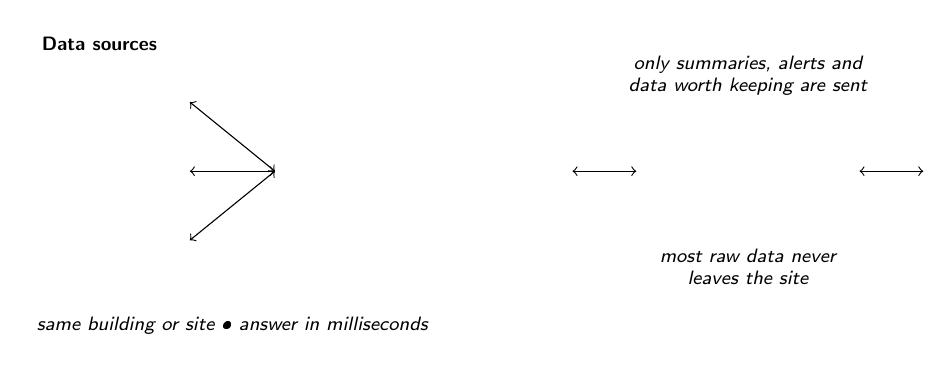
\begin{tikzpicture}[x=1.35cm,y=1.35cm,rounded corners=2pt]
  \tikzset{lbl/.append style={font=\sffamily\scriptsize\hyphenpenalty10000}}
  \node[lbl,font=\sffamily\scriptsize\bfseries] at (0.95,3.75) {Data sources};
  \B{0.1,2.95}{1.8,3.45}{Camera}
  \B{0.1,2.30}{1.8,2.80}{Sensor}
  \B{0.1,1.65}{1.8,2.15}{Machine / phone}
  \foreach \y in {3.20,2.55,1.90} {\draw[<->] (1.8,\y) -- (2.6,2.55);}
  \B[line width=1.2pt]{2.6,1.45}{5.4,3.65}{\textbf{Edge node}\\a computer placed\\beside the data source\\(gateway or small server)\\[3pt]filters, analyses and\\acts on the data at once}
  \node[lbl,font=\sffamily\scriptsize\itshape,align=center] at (2.2,1.10)
    {same building or site \textbullet{} answer in milliseconds};
  \B[dashed]{6.0,2.05}{8.1,3.05}{Wide-area network\\/ Internet\\(shared, slower)}
  \draw[<->] (5.4,2.55) -- (6.0,2.55);
  \draw[<->] (8.1,2.55) -- (8.7,2.55);
  \B[line width=1.2pt]{8.7,1.45}{11.4,3.65}{\textbf{Cloud data centre}\\hundreds or thousands\\of kilometres away\\[3pt]long-term storage,\\reports, and training of\\machine learning models}
  \node[lbl,font=\sffamily\scriptsize\itshape,align=center] at (7.05,3.45)
    {only summaries, alerts and\\data worth keeping are sent};
  \node[lbl,font=\sffamily\scriptsize\itshape,align=center] at (7.05,1.65)
    {most raw data never\\leaves the site};
\end{tikzpicture}
\caption{Basic working model of edge computing}
\label{fig:edge-basic}
\end{figure}

\begin{notebox}
Edge computing does not replace cloud computing. The two work together: the
edge handles what must be fast, private or independent of the network, and
the cloud handles what needs large storage, heavy computation or a view
across many sites.
\end{notebox}

\subsection{Where the Edge Is}

``The edge'' is not one fixed place. Depending on the application the
computing may sit at any of the following points, and a real system often
uses more than one of them~\rc{ref:lea}.

\begin{itemize}
  \item \textbf{On the device itself} --- a camera that recognises a number
        plate inside the camera, or a watch that counts steps without help
        from a phone
  \item \textbf{On a gateway at the site} --- one small computer in a
        factory, farm or hospital that serves all the devices around it
  \item \textbf{At the network operator's premises} --- a small data centre
        at a mobile base station, serving every user connected to it. This
        arrangement is called multi-access edge computing~\rc{ref:etsi}
\end{itemize}

The term \textbf{fog computing} is often met alongside edge computing. It
describes the same idea with the emphasis on an intermediate layer of
gateways and regional nodes between the devices and the cloud, rather than on
the devices themselves~\rc{ref:bonomi}. For this course the two may be treated
as the same approach seen from slightly different distances.

%%%%%%%%%%%%%%%%%%%%%%%%%%%%%%%%%%%%%%%%%%%%%%%%%%%%%%%%%%%%%%%%%%%%%%%%%%%%%%%%%%%%%%%%%%%%%%
\section{Need for Edge Computing}

Cloud computing solved the problem of obtaining capacity without owning it.
It did not solve the problem of distance. Sending data to a distant data
centre takes time, consumes network capacity, and fails when the network
fails. The reasons for computing at the edge follow from these
facts~\rcc{ref:shi}{ref:satya}.

\begin{itemize}
  \item \textbf{Latency} --- some decisions cannot wait for a round trip to a
        data centre. A self-driving vehicle that must brake, a robot arm that
        must stop before it injures someone, or a game that must respond to a
        movement, needs an answer within a few milliseconds. A round trip to
        a cloud region typically costs tens of milliseconds, and more when
        the network is busy.
  \item \textbf{Bandwidth} --- sending everything is often simply too much
        data. One high-definition camera produces roughly 4~Mbps of video, so
        a campus with 100 cameras would need about 400~Mbps of upload
        capacity, continuously, only to send video that is almost entirely
        uneventful. An edge node can watch all 100 streams locally and send
        on only the few seconds that matter.
  \item \textbf{Intermittent connectivity} --- ships, mines, farms, oil rigs
        and rural clinics do not have a dependable link to the Internet. Work
        that depends on reaching the cloud stops when the link does; work
        done at the edge continues and synchronises later.
  \item \textbf{Privacy and regulation} --- medical records, classroom
        footage and factory process data may be sensitive, or may be required
        by law to stay within the premises or the country. Processing locally
        and sending only anonymous summaries keeps the raw data where it
        belongs.
  \item \textbf{Cost} --- network transfer and cloud storage are charged by
        volume, so discarding uninteresting data at the edge reduces both
        bills.
  \item \textbf{Scale} --- the number of connected devices grows faster than
        the capacity of the links to the cloud, so a design that forwards
        everything to the centre becomes harder to sustain as devices are
        added~\rcc{ref:lea}{ref:hwangiot}.
\end{itemize}

%%%%%%%%%%%%%%%%%%%%%%%%%%%%%%%%%%%%%%%%%%%%%%%%%%%%%%%%%%%%%%%%%%%%%%%%%%%%%%%%%%%%%%%%%%%%%%
\section{Edge Computing Architecture}

An edge computing system is usually described as a set of tiers, or layers,
arranged by distance from the data~\rcc{ref:lea}{ref:bonomi}.
Figure~\ref{fig:edge-arch} shows the four tiers and what each one does. It is
read from the bottom, where the data is created, to the top, where the cloud
sits.

\begin{figure}[!htb]
\centering
\begin{tikzpicture}[x=1.5cm,y=1.4cm,rounded corners=2pt]
  \tikzset{lbl/.append style={font=\sffamily\scriptsize}}
  \B[line width=1.2pt][text width=10.2cm,font=\sffamily\scriptsize\hyphenpenalty10000\exhyphenpenalty10000]{0.2,4.15}{7.4,5.15}%
    {\textbf{Cloud tier} --- large data centre\\
     long-term storage \textbullet{} reports and dashboards \textbullet{}
     training of machine learning models \textbullet{} view across all sites}
  \B[line width=1.2pt][text width=10.2cm,font=\sffamily\scriptsize\hyphenpenalty10000\exhyphenpenalty10000]{0.2,2.85}{7.4,3.85}%
    {\textbf{Regional (fog) tier} --- operator or campus micro data centre\\
     combines data from several sites \textbullet{} keeps it for days
     \textbullet{} runs heavier analysis}
  \B[line width=1.2pt][text width=10.2cm,font=\sffamily\scriptsize\hyphenpenalty10000\exhyphenpenalty10000]{0.2,1.55}{7.4,2.55}%
    {\textbf{Edge tier} --- gateway or small server at the site\\
     filters and summarises data \textbullet{} real-time decisions and control
     \textbullet{} local storage \textbullet{} runs trained models}
  \B[line width=1.2pt][text width=10.2cm,font=\sffamily\scriptsize\hyphenpenalty10000\exhyphenpenalty10000]{0.2,0.25}{7.4,1.25}%
    {\textbf{Device tier} --- sensors, cameras, machines, phones, vehicles\\
     the data is created here \textbullet{} simple devices only measure,
     capable ones process a little themselves}
  \foreach \y in {1.25,2.55,3.85} {
    \draw[<->] (1.8,\y) -- (1.8,\y+0.30);
    \draw[<->] (5.8,\y) -- (5.8,\y+0.30);
  }
  \node[lbl,font=\sffamily\scriptsize\itshape] at (3.8,1.40) {local network};
  \node[lbl,font=\sffamily\scriptsize\itshape] at (3.8,2.70) {site link};
  \node[lbl,font=\sffamily\scriptsize\itshape] at (3.8,4.00) {wide-area network};
  \draw[->,line width=1.1pt,sharp corners] (7.9,0.35) -- (7.9,5.05);
  \node[lbl,rotate=90,anchor=south] at (7.8,2.7)
    {distance, latency and computing power increase};
  \draw[->,line width=1.1pt,sharp corners] (8.7,5.05) -- (8.7,0.35);
  \node[lbl,rotate=90,anchor=north] at (8.8,2.7) {volume of data increases};
\end{tikzpicture}
\caption{Architecture of an edge computing system: four tiers, from the
devices that create the data to the cloud}
\label{fig:edge-arch}
\end{figure}

\subsection{The Tiers}

\begin{itemize}
  \item \textbf{Device tier} --- the sensors, cameras, machines, vehicles and
        phones that produce the data. A simple sensor only measures and
        reports; a more capable device performs a little processing itself,
        such as discarding a reading that has not changed.
  \item \textbf{Edge tier} --- one or more computers at the site: a gateway,
        an industrial PC or a small server. This tier receives data from the
        devices over a local network, filters and summarises it, takes the
        decisions that must be immediate, keeps a short history locally, and
        forwards what is worth forwarding.
  \item \textbf{Regional or fog tier} --- a micro data centre belonging to the
        organisation or to the network operator and serving several sites. It
        combines their data, keeps it for days or weeks, and runs analysis
        that is too heavy for a gateway. Small systems often leave this tier
        out and connect the edge tier directly to the cloud.
  \item \textbf{Cloud tier} --- the large data centre studied in the previous
        topic. It provides effectively unlimited storage and computing power,
        a view across every site, and the place where machine learning models
        are trained before being sent down to the edge to be used.
\end{itemize}

\subsection{How Work Is Divided Between the Tiers}

Two quantities change as one moves up the diagram, and the design follows
from them. The volume of data is largest at the bottom, because every device
produces data continuously, and it shrinks at each tier as data is filtered
and summarised. Computing power, storage and distance all grow towards the
top. The working rule is therefore simple: perform a task at the lowest tier
that is able to perform it, and send upward only what the higher tier
genuinely needs~\rc{ref:shi}.

A traffic camera illustrates the division. The camera captures video (device
tier). The edge node watches that video, recognises a vehicle crossing a red
light and raises an alert within a fraction of a second, discarding the rest
(edge tier). Each evening it uploads the recorded violations and a count of
vehicles per hour to the cloud, which stores them, prepares reports for the
whole city, and periodically trains an improved recognition model that is
then sent back to the edge nodes (cloud tier).

%%%%%%%%%%%%%%%%%%%%%%%%%%%%%%%%%%%%%%%%%%%%%%%%%%%%%%%%%%%%%%%%%%%%%%%%%%%%%%%%%%%%%%%%%%%%%%
\section{Cloud versus Edge Computing}

The two are partners rather than rivals, but they differ in almost every
practical respect~\rcc{ref:shi}{ref:buyyacloud}.

\begin{center}
\begin{tabularx}{\textwidth}{@{}p{3.2cm}LL@{}}
\toprule
\textbf{Aspect} & \textbf{Cloud computing} & \textbf{Edge computing} \\
\midrule
Location of processing & Large data centres, far from the user & Close to
  where the data is produced \\
Typical response time & Tens of milliseconds or more & A few milliseconds \\
Computing power & Very large and elastic & Limited by what fits at the site \\
Storage & Effectively unlimited & Small; usually a short local history \\
Data sent over the network & All of it & Only summaries and important
  events \\
Works without the Internet & No & Yes, for local tasks \\
Privacy of raw data & Leaves the premises & Can stay on the premises \\
Cost pattern & Pay for capacity, transfer and storage used & Pay once for the
  equipment, then little transfer cost \\
Scope of view & Every site together & One site or one device \\
Suitable work & Training models, long-term storage, reports across sites &
  Immediate decisions, filtering, local control \\
Management & One provider manages the hardware & Many small units in many
  places must be managed \\
\bottomrule
\end{tabularx}
\end{center}

%%%%%%%%%%%%%%%%%%%%%%%%%%%%%%%%%%%%%%%%%%%%%%%%%%%%%%%%%%%%%%%%%%%%%%%%%%%%%%%%%%%%%%%%%%%%%%
\section{Applications}

\begin{itemize}
  \item \textbf{Industrial automation} --- machines on a production line are
        monitored for vibration, temperature and current, and an edge node
        stops a machine or raises a maintenance alert before a fault becomes
        a breakdown
  \item \textbf{Autonomous and assisted driving} --- a vehicle interprets its
        cameras and sensors on board, because braking cannot wait for a reply
        from a data centre~\rc{ref:satya}
  \item \textbf{Video surveillance and traffic management} --- cameras and
        edge nodes detect events locally and send only the relevant clips
        instead of streaming everything
  \item \textbf{Healthcare} --- bedside monitors raise alarms locally, and
        patient data is summarised before anything leaves the hospital
  \item \textbf{Agriculture} --- soil, weather and crop-health sensors are
        processed on a farm gateway, which keeps working where network
        coverage is poor
  \item \textbf{Smart cities and utilities} --- street lighting, water
        distribution and electricity meters are controlled locally, with
        readings summarised for the central system
  \item \textbf{Retail} --- shelf cameras, billing counters and stock sensors
        are processed in the store, so that it continues to operate even if
        the link to the head office is lost
  \item \textbf{Content delivery and gaming} --- copies of popular videos,
        pages and game servers are kept near users so that they load quickly
        and the central servers carry less load
\end{itemize}

%%%%%%%%%%%%%%%%%%%%%%%%%%%%%%%%%%%%%%%%%%%%%%%%%%%%%%%%%%%%%%%%%%%%%%%%%%%%%%%%%%%%%%%%%%%%%%
\section{Advantages and Limitations}

\textbf{Advantages}
\begin{itemize}
  \item Responses in milliseconds, because the data does not travel far
  \item Much less network traffic, and lower transfer and storage cost
  \item Continues to work when the connection to the cloud is lost
  \item Sensitive data can be kept within the premises
  \item Capacity grows naturally as devices and sites are added
\end{itemize}

\textbf{Limitations}
\begin{itemize}
  \item Computing power, memory and storage at a site are limited compared
        with a data centre
  \item Many small units spread over many locations are harder to update,
        monitor and repair than one data centre
  \item Physical security is weaker: equipment sits in factories, streets and
        vehicles rather than in a guarded building
  \item Devices and gateways from different makers must be made to work
        together, and standards are still settling
  \item Only a local view is available, so conclusions that need data from
        every site still require the cloud
\end{itemize}

%%%%%%%%%%%%%%%%%%%%%%%%%%%%%%%%%%%%%%%%%%%%%%%%%%%%%%%%%%%%%%%%%%%%%%%%%%%%%%%%%%%%%%%%%%%%%%
\section{Review Questions}

\textbf{CO1 --- Describe modern computing approaches and their
characteristics}\\
\textit{Bloom's Level L1 --- Remember, L2 --- Understand}

\begin{enumerate}[label=\arabic*.]
  \item Define edge computing. Where exactly is ``the edge'' in a computing
        system?
  \item Define latency and bandwidth, and state the unit in which each is
        measured.
  \item With a neat diagram, explain the basic working model of edge
        computing.
  \item State any four reasons why edge computing is needed.
  \item Explain, with one example each, how edge computing helps when the
        network connection is unreliable and when the data is sensitive.
  \item With a neat diagram, explain the architecture of an edge computing
        system, naming each tier and stating what it does.
  \item What is a gateway in an edge computing system, and what work does it
        perform?
  \item Differentiate between cloud computing and edge computing with respect
        to location of processing, response time, storage and network usage.
  \item Explain why edge computing is described as a partner of cloud
        computing rather than a replacement for it.
  \item What is fog computing, and how is it related to edge computing?
  \item List any five applications of edge computing, stating in each case
        why the processing must be done locally.
  \item State any four limitations of edge computing.
  \item Describe how a traffic camera system would divide its work between
        the device, edge and cloud tiers.
\end{enumerate}

%%%%%%%%%%%%%%%%%%%%%%%%%%%%%%%%%%%%%%%%%%%%%%%%%%%%%%%%%%%%%%%%%%%%%%%%%%%%%%%%%%%%%%%%%%%%%%
\section{References and Further Reading}

Items~\ref{ref:lea} to~\ref{ref:hwangiot} are the prescribed books for this
module; chapter numbers are indicative. Items~\ref{ref:shi}
to~\ref{ref:bonomi} are the papers from which the definitions and the tiered
architecture are taken, and item~\ref{ref:etsi} is the standards site for
edge computing in mobile networks.

\begin{enumerate}[label={[\arabic*]},ref=\arabic*,leftmargin=2.2em]
  \item\label{ref:lea} P.~Lea, \textit{IoT and Edge Computing for
        Architects}, 2nd Edition, Packt Publishing, 2020 --- Reference
        Book~1 for this course; chapters on edge computing and edge
        architecture.
  \item\label{ref:buyyacloud} R.~Buyya, C.~Vecchiola, S.~T.~Selvi,
        S.~Poojara and S.~N.~Srirama, \textit{Mastering Cloud Computing}, 2nd
        Edition, Morgan Kaufmann, 2026 --- Text Book~2 for this course; used
        here for the cloud side of the comparison.
  \item\label{ref:hwangiot} K.~Hwang, G.~C.~Fox and J.~J.~Dongarra,
        \textit{Distributed and Cloud Computing: From Parallel Processing to
        the Internet of Things}, Morgan Kaufmann, 2012 --- Text Book~1 for
        this course; used here for sensors, devices and the growth in the
        number of connected things.
  \item\label{ref:shi} W.~Shi, J.~Cao, Q.~Zhang, Y.~Li and L.~Xu, ``Edge
        Computing: Vision and Challenges'', \textit{IEEE Internet of Things
        Journal}, vol.~3, no.~5, pp.~637--646, 2016.
  \item\label{ref:satya} M.~Satyanarayanan, ``The Emergence of Edge
        Computing'', \textit{IEEE Computer}, vol.~50, no.~1, pp.~30--39,
        2017.
  \item\label{ref:bonomi} F.~Bonomi, R.~Milito, J.~Zhu and S.~Addepalli,
        ``Fog Computing and Its Role in the Internet of Things'',
        \textit{Proceedings of the First MCC Workshop on Mobile Cloud
        Computing}, ACM, 2012, pp.~13--16.
  \item\label{ref:etsi} ETSI, Multi-access Edge Computing (MEC).
        \url{https://www.etsi.org/technologies/multi-access-edge-computing}
\end{enumerate}

\end{document}